\chapter{Introduction}
\label{chap:introduction}

Artificial intelligence is a powerful tool for tackling difficult problems,
from playing chess to driving autonomous cars.
This thesis explores how we can use artificial intelligence to optimize
learning of introductory programming.
%This thesis explores how can be artificial intelligence used to optimize
%learning of introductory programming.

Adaptive learning systems have been already successfully used in many domains
\cite{alg.evaluation-geography} (+CITE).
However, the most popular introductory programming tutorials
(Hour of Code) still use a fixed sequence of tasks for everybody,
leading to a suboptimal experience.
Aritificial intelligence can be used to personalize the sequence of tasks
for each student.
By giving students tasks of optimal difficulty, neither too easy, nor too
difficult, we help them to achieve complete immersion into the problem solving
activity, which is known as a \emph{state of flow} \cite{flow}
(figure \ref{fig:flow}).
The state of flow is essential for the optimal learning experience
\cite{adaptive-practice}.

\begin{figure}[htb]
  \centering
  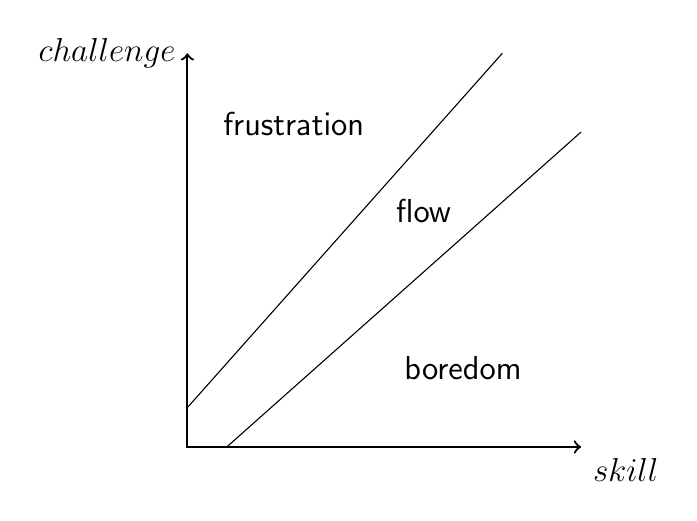
\begin{tikzpicture}[font=\sffamily,xscale=5, yscale=5]
  \large
  %\draw [lightgray, fill=gray] (0,0) -- (0.1,0) -- (1,0.8) -- (0.8,1) -- (0,0.1) -- (0,0);
  \draw (0.1,0) -- (1,0.8);
  \draw (0,0.1) -- (0.8,1);
  \draw [thick, <->] (0,1) node [left] {$challenge$} -- (0,0) -- (1,0) node [below right] {$skill$};
  \node at (0.27,0.82) {frustration};
  \node at (0.6,0.6) {flow};
  \node at (0.7,0.2) {boredom};
  \end{tikzpicture}
  \caption{Relationship between challenge and skill.}
  \label{fig:flow}
\end{figure}

%TODO: related areas
%- introductory programming learning
%- adaptive learning / intelligent tutoring systems
%- recommendation systems (with performance instead of ratings)
%- HCI, (software learnability)
%- games design \cite{book-of-lenses}

How can be domain and students of introductory programming modelled?
Which algorithms to use for task recommendation and mastery learning?
How to evaluate components of the adaptive learning system?
%How to evaluate if the adaptivity of the system helps to improve learning and engagement?
% TODO: Make sure these questions are answered in the text (or remove them).
To answer these questions, we not only look at the existing systems
and research, but we also develop our own adaptive learning system for
introductory programming\footnote{Available at \url{en.robomise.cz}}
(figure \ref{fig:robomission-task1}).
Devopment of this system helps us to better understand related challenges
and enable us to collect data for analyses we need to support or reject our hypotheses.
% TODO: And are there such hypotheses in the thesis?

% TODO: English screenshot.
\imgW[0.9]{robomission-task1}%
  {RoboMission -- application for learning programming.}

We first look at how the introductory programming is currently taught
(chapter \ref{chap:learning-programming}),
and explore relevant techniques of adaptive learning (chapter \ref{chap:adaptive-learning}).
%We focus on models of domain and student for introductory programming,
%algorithms for task recommendation and mastery learning,
%and evaluation of the system and its components.
Then, we describe a new game designed for learning introductory programming
(chapter \ref{chap:design-of-game}),
adpativity of our system (chapter \ref{chap:design-of-adaptivity}),
and its implementation (chapter \ref{chap:implementation-of-robomission}).
We conclude the thesis with analyses of collected data
(chapter \ref{chap:analysis}).
